\section{Results}
% \addcontentsline{toc}{section}{Results}
\fancyhead[R]{Results}

\subsection{Model Performance}
\label{sec:Model Performance}

This chapter presents the performance metrics of the developed model before and after the hyperparameter tuning. The model was evaluated at different EC levels to assess its accuracy, recall, and F1 score. These metrics provide insight into the model's initial performance and highlight areas for potential improvement through hyperparameter tuning. The metrics are calculated based on the model's predictions and the actual enzyme classes in the test dataset. For better comparability, the model's performance is evaluated at each EC level separately. Accuracy, Recall and F1 are used for a better comparison of the performance with other models.

\begin{table}[!htbp]
    \centering
    \begin{tabular}{@{}llll@{}}
    \toprule
    \textbf{EC Level} & \textbf{Accuracy} & \textbf{Recall} & \textbf{F1} \\ \midrule
    1                 & 0.94              & 0,94            & 0,93        \\
    2                 & 0,90              & 0,90            & 0,90        \\
    3                 & 0,94              & 0,94            & 0,93        \\
    4                 & 0,75              & 0,75            & 0,72        \\ \bottomrule
    \end{tabular}
    \caption{Model Performance before Hyperparameter tuning and Resampling}
    \label{tab:performance-before-tuning}
\end{table}

As shown in the table above, the model performs well at the first three levels of the Enzyme Commission (EC) hierarchy, with high accuracy, recall, and F1 score. However, the model's performance decreases at the fourth EC level, where the classification becomes more specific and challenging. The drop in accuracy, recall, and F1 score at this level indicates that the model struggles to predict the most detailed enzyme classes accurately. Predicting the 4th EC Level is significantly more challenging than predicting higher levels due to the need to select from approximately 7000 classes \ref{tab:ec-level-distribution}, increasing the difficulty of accurate prediction. The model's performance at the fourth EC level suggests that further optimization is needed to improve its predictive power for more specific enzyme classes. To increase the model performance the dataset was edited with the help of the RandomUnderSampler as shown in chapter \ref{sec:Data Preprocessing}. The model was retrained on the resampled dataset with no further changes to the model architecture and parameters. The results of the model performance after resampling are shown in the following table:

\begin{table}[!htbp]
    \centering
    \begin{tabular}{@{}llll@{}}
    \toprule
    \textbf{EC Level} & \textbf{Accuracy} & \textbf{Recall} & \textbf{F1} \\ \midrule
    1                 & 0.91              & 0,91            & 0,91        \\
    2                 & 0,94              & 0,92            & 0,94        \\
    3                 & 0,96              & 0,96            & 0,96        \\
    4                 & 0,80              & 0,80            & 0,78        \\ \bottomrule
    \end{tabular}
    \caption{Model Performance after Resampling}
    \label{tab:performance-after-resampling}
\end{table}

The performance metrics still show a significant decrease in accuracy, recall, and F1 score at the fourth EC level. The results suggest that the model performs well at higher levels of the EC hierarchy (levels 1 to 3), but there is a notable decrease in performance at the most specific level (level 4). This suggests that there is room for improvement, particularly in fine-tuning the model for more specific classifications. To optimize the predictions even further, the model was fine-tuned using hyperparameter tuning. The results of the model performance after hyperparameter tuning are shown in the following table:

\begin{figure}[!h]
    \centering
    \begin{minipage}[t]{\textwidth}
    \caption{Model Performance before and after Hyperparameter tuning}
    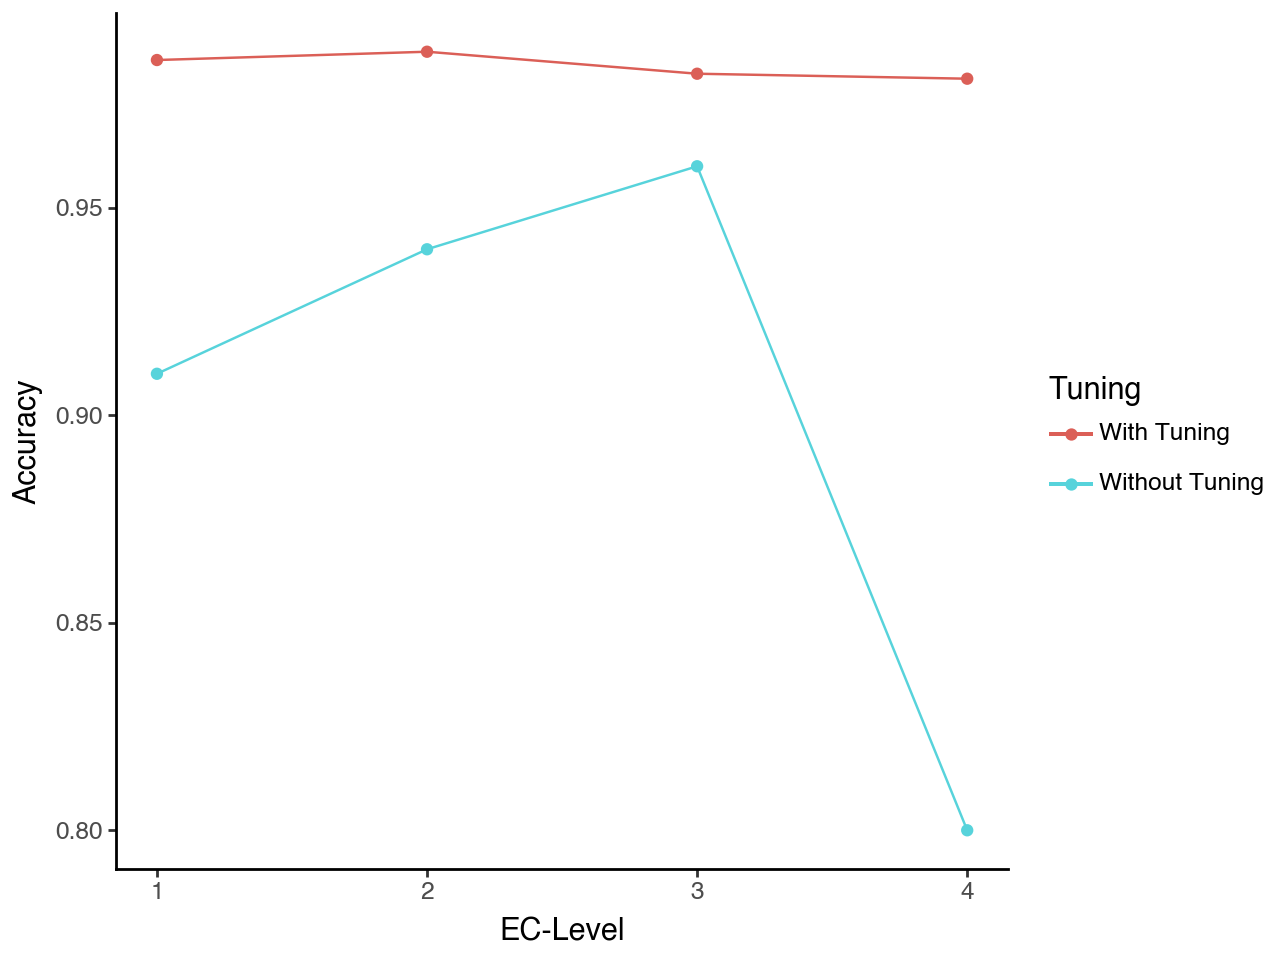
\includegraphics[scale=0.55]{img/model-performance-comparison.png}
    \source{Own illustration}
    \label{fig:performance-comparison}
    \end{minipage}
\end{figure}

The hyperparameter tuning has improved the model's performance at the fourth EC level, with a significant increase in accuracy, recall, and F1 score. This indicates that the model is better able to predict the most specific enzyme classes after the fine-tuning process. On the other hand, the model's performance at the first three levels remains consistent, suggesting that the hyperparameter tuning has not significantly impacted the model's performance at these levels. Since the increase in performance is only around 10 percent, further optimization may be required to enhance the model's predictive power at the fourth EC level. This could involve refining the model architecture, increasing the size of the training dataset, or incorporating additional features to improve the model's ability to predict specific enzyme classes. A possible approach could be to integrate anchor points based on protein sequences to get a more accurate prediction of the fourth EC level. Dalkiran et al. (2018) have shown that anchor points can significantly improve the prediction accuracy of enzyme classes, particularly at the most specific level. \autocite{dalkiranECPredToolPrediction2018a}

\pagebreak

\subsection{Comparative Analysis with Existing Models}
\label{sec:Comparative Analysis with Existing Models}

To evaluate the performance of the proposed model, a comparative analysis was conducted against existing state-of-the-art models: DeepRE, EzyDeep, and HecNet. The comparison focuses on the prediction accuracy across the four levels of the Enzyme Commission (EC) classification system. All models were evaluated on the same dataset provided by COFACTOR, ensuring a fair and consistent comparison. \autocite{zhangCOFACTORImprovedProtein2017}

\begin{figure}[!h]
    \centering
    \begin{minipage}[t]{\textwidth}
    \caption{Comparison of Accuracy with other models}
    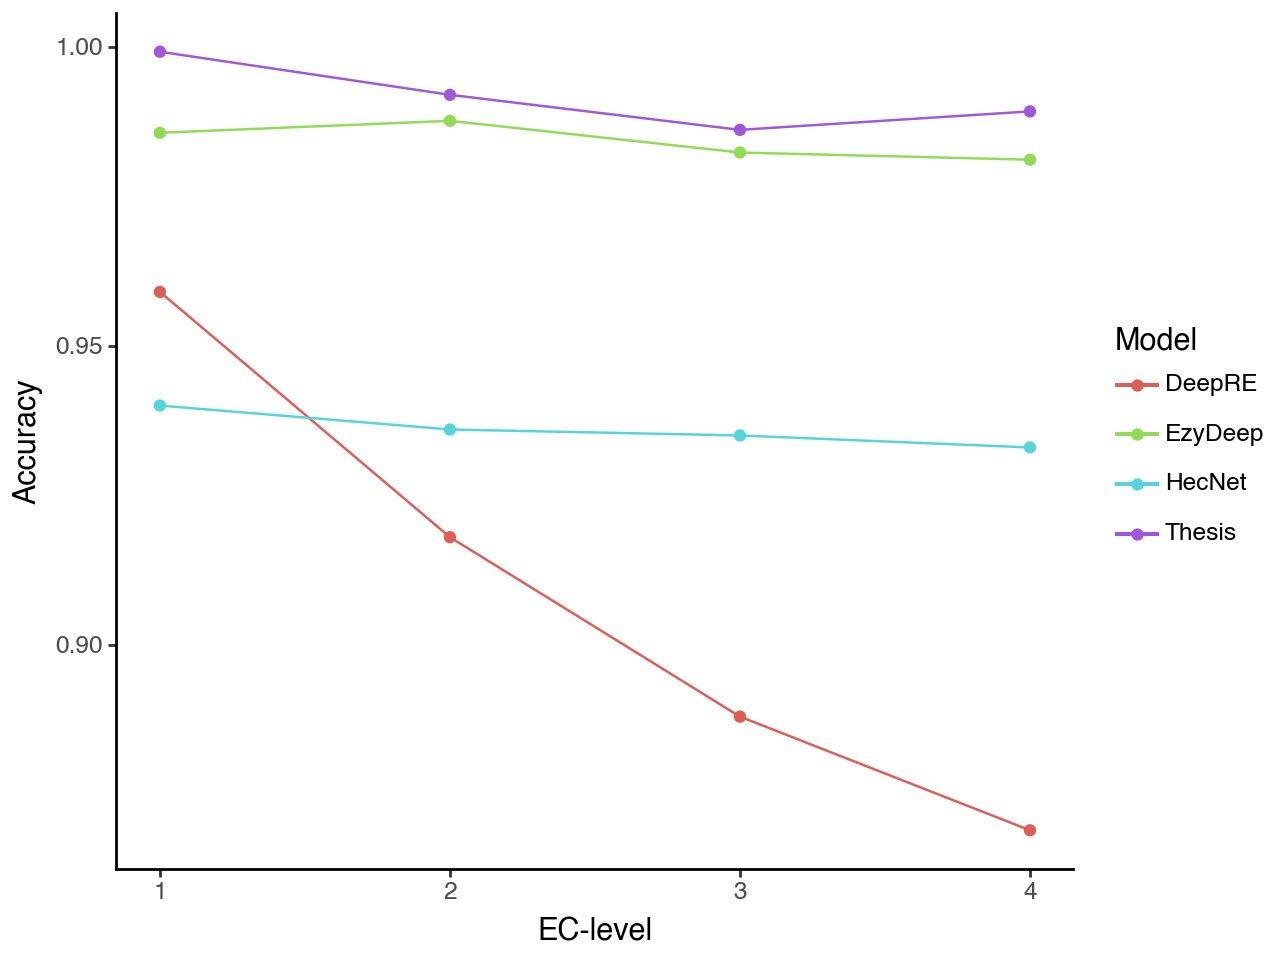
\includegraphics[scale=0.7]{img/comparison-with-other-models.png}
    \source{Own illustration}
    \label{fig:comparison-with-other-models}
    \end{minipage}
\end{figure}

As shown in the figure above, the proposed model outperforms existing models at the all levels of the EC hierarchy, with a higher accuracy. The model's performance at the first three levels is significantly better than existing models, demonstrating its superior predictive power. This suggests that the model's focus on ligand-binding sites has contributed to its high accuracy and precision in predicting enzyme classes. The targeted approach to enzyme classification has proven to be more effective than traditional methods that utilize the entire protein sequence. The model's emphasis on ligand-binding sites enables it to capture the functional aspects of enzymes more accurately. This targeted approach reduces computational complexity and enhances prediction accuracy, making it a valuable tool for enzyme classification and prediction.

The model's performance at the fourth EC level is comparable with EzyDeep, indicating that it can predict specific enzyme classes with similar accuracy. Although the performance of all models declines at this level due to the increased complexity, the Thesis model still achieves the highest accuracy. This indicates its ability to manage detailed and specific enzyme classifications effectively. Maintaining high accuracy at this level is critical for understanding the enzyme's catalytic activity.

Despite these advancements, there is still room for improvement. Further refinement in balancing techniques could improve model performance on underrepresented classes. A more extensive Hyperparameter tuning could also enhance the model's predictive power, particularly at the most specific classification levels. In addition to that, incorporating more diverse biochemical and environmental data could enhance model accuracy, especially at the most specific classification levels. The methods to enhance the model's performance are discussed in the section \ref{sec:Final Remarks and Future Work} in detail.

\subsection{Interpretation of Model Predictions}
\label{sec:Interpretation of Model Predictions}

The Deep Learning model developed in this study predicts enzyme classes with a high degree of accuracy, particularly at the first three levels of the Enzyme Commission (EC) classification hierarchy. The focus on ligand-binding sites has significantly contributed to the precision of the prediction at the fourth level, which is the most challenging due to the high number of classes and the complexity of enzyme functions. Predicting the fourth level is crucial for understanding the specific functions of enzymes that are involved in certain metabolic pathways, such as pesticide degradation. The model's performance at this level provides valuable insights into the enzyme's catalytic activity and substrate specificity, which are essential for designing effective products for agricultural applications.

However, the model's performance decreases at the fourth EC level, where the classification becomes highly specific. This drop in accuracy highlights the complexity and diversity of enzyme functions at this detailed level. This shows that the model needs further optimization to accurately predict the most specific enzyme classes. Integrating additional biochemical and environmental data, as well as refining the model architecture, could address the challenges associated with this level of specificity. Collaborative efforts with experimental biologists will be essential for validating and expanding the model’s applicability. In addition to that, the model's performance can be further improved by increasing the size of the training dataset and incorporating more diverse enzyme sequences. This will help the model learn more about the subtle differences between enzyme classes and improve its predictive power.

The model's emphasis on ligand-binding sites offers a \textit{novel} and effective approach to enzyme classification. By concentrating on these specific regions, the model accurately captures the functional aspects of enzymes that are most relevant to their interaction with pesticides. This targeted approach reduces computational complexity and enhances prediction accuracy, providing more reliable insights into enzyme activity. The ligand-binding site predictions enable the identification of key residues involved in pesticide degradation. Understanding these critical interaction points can inform the design of more effective bioremediation strategies and the development of enzyme-based products for agricultural applications. 